\documentclass{beamer}
\usetheme{Madrid}
\usepackage{tikz}
\usepackage{graphicx}
\usepackage{subcaption}
\usepackage{xcolor,colortbl}
\usepackage{pgfplots}
\usepackage{bchart}
\usetikzlibrary{shapes}
 
\tikzstyle{golla} = [circle,draw]
\definecolor{Gray}{gray}{0.85}
\definecolor{LightCyan}{rgb}{67, 250, 243}
 
 
\title[beamer class]{Can Women Break the Glass Ceiling?: An Analysis of \#MeToo Hashtagged Posts on Twitter}
\author[muntaka,adiba,sworna]{1605097, 1605106, 1605114}
\institute[BUET]{Bangladesh University of Engineering and Technology}
\date{\today}
 
\begin{document}
    \maketitle
   
    \begin{frame}{Table of Contents}
        \tableofcontents
       
    \end{frame}
   
    \begin{frame}
        \frametitle{Introduction}
        \begin{itemize}
            \item October 15, 2017 : Tweeter news feed exploded by a tweet  of Alyssa Milano  \pause
            \item Women all over the world shared their story of sexual harassment and sexual assault in social media with a hashtag \#MeToo\pause
            \item More than 4.5 million posts within 24 hours \pause
           
        \end{itemize}
    \end{frame}
    \begin{frame}
        \frametitle{Previous Works}
       
        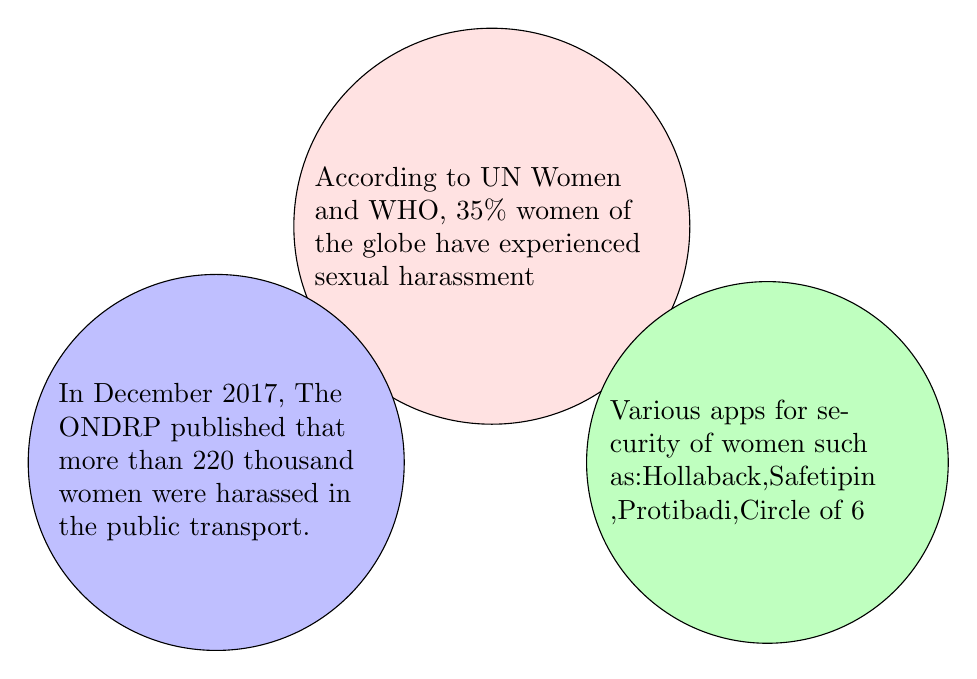
\begin{tikzpicture}
        \centering
        \node[golla,fill = pink!45, text width=4.5cm] at(6.5,3.8)(point1) {According to UN Women and WHO, 35\% women of the globe have experienced sexual harassment};\pause
        \node[golla,fill=blue!25,text width=4cm]at(3,0.8)(point2){In December 2017, The ONDRP published that more than 220 thousand women were harassed in the public transport.};\pause
        \node[golla,fill=green!25,text width=4cm]at(10,0.8)(point3){Various apps for security of women such as:Hollaback,Safetipin
            ,Protibadi,Circle of 6};
       
        \end{tikzpicture}
       
    \end{frame}
    \begin{frame}
        \frametitle{Data Collection}
        \centering
        \begin{tabular}{|l|l|l|l|l|}
            \hline
            \rowcolor{LightCyan}
            \textbf{City} & \textbf{\#Tweets} & \textbf{Male} & \textbf{Female} & \textbf{Female(\%)}   \\
           
            \hline
            Dallas & 1249 & 144 & 471 & 76.59 \\
            \hline
            Dhaka & 82 & 32 &  22 & 40.74  \\
            \hline
            Indianapolis & 1203 & 180 & 452 & 71.52  \\
            \hline
            Kansan City & 448 & 61 & 208 & 77.32  \\
            \hline
            Karachi & 250 & 44 & 55 & 55.56  \\
            \hline
            Mumbai & 2778 & 724 & 674 & 48.21  \\
            \hline
            New York & 1878 & 267 & 754 & 73.85  \\
            \hline
            North Dakota & 110 & 18 & 34 & 65.38  \\
            \hline
            Portland & 849 & 146 & 316 & 68.4  \\
            \hline
            Saint Louis & 619 & 92 & 224 & 70.89  \\
            \hline
            Tehran & 114 & 13 & 32 & 71.11  \\
            \hline
           
           
        \end{tabular}
       
    \end{frame}
    \begin{frame}
        \frametitle{Analysis}
        \begin{itemize}
            \item \textbf{Age and Gender Distribution}\pause
        \end{itemize}
        \begin{figure}[h]
            \centering
            \begin{subfigure}{0.45\textwidth}
                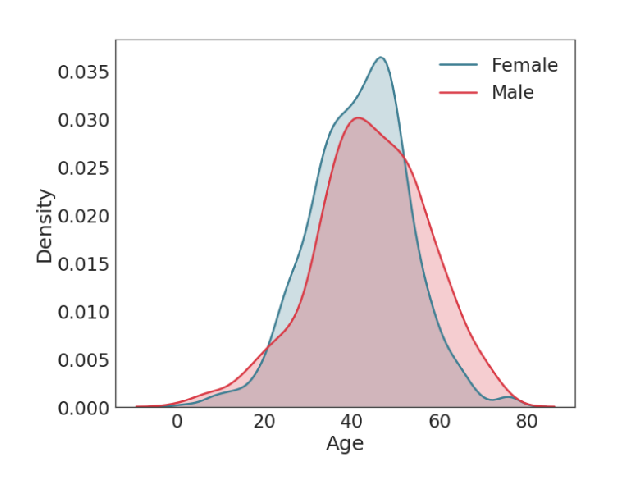
\includegraphics[width=0.85\textwidth]{SS1}
                %\includegraphics[width=0.85\textwidth]{p1.png}
                \caption{US}
            \end{subfigure} \pause
            ~
            \begin{subfigure}{0.45\textwidth}
                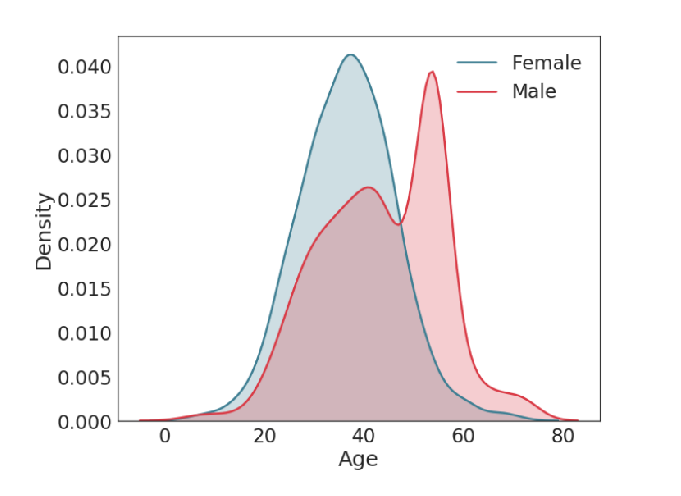
\includegraphics[width=0.85\textwidth]{SS2}
                \caption{Asia}
            \end{subfigure}
            \caption{Age distribution of female and male users}
        \end{figure}
       
    \end{frame}
   
   
   
   
    \begin{frame}
        \frametitle{Frequency of different harassment categories}
        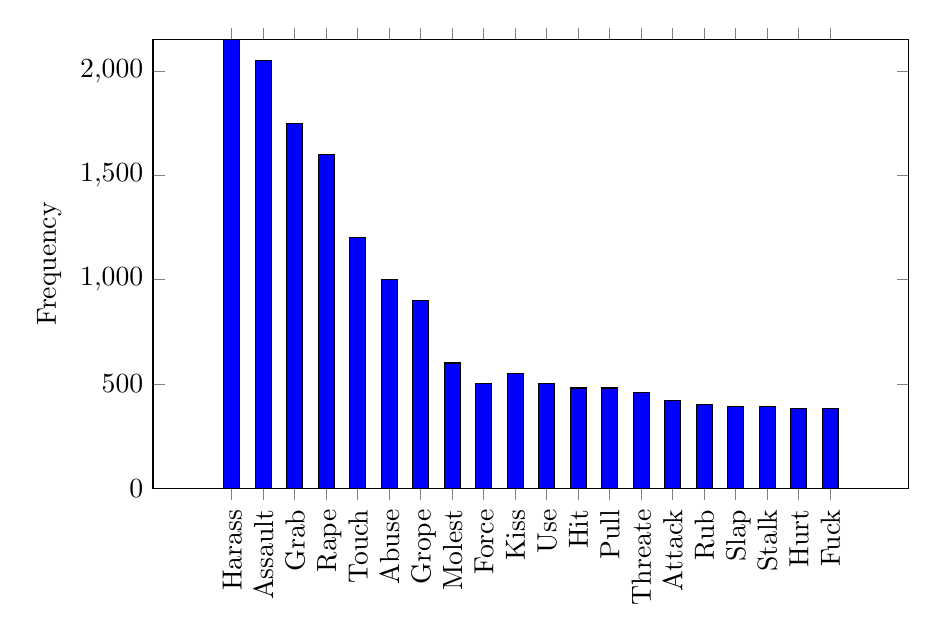
\begin{tikzpicture}
        \begin{axis}[
        ybar,
        bar width=.2cm, % Width of the bar
        x=.4cm, % Distance between the centers of the bars
        enlarge x limits={abs=1cm}, % The distance between the center of the first bar and the left edge
        enlarge y limits=false,
        ymin=0,
        xtick=data,
        xlabel=,
        symbolic x coords={Harass, Assault, Grab,Rape,Touch,Abuse,Grope,Molest,Force,Kiss,Use,Hit,Pull,
            Threate,Attack,Rub,Slap,Stalk,Hurt,Fuck},
        xtick=data,
        ylabel=Frequency,
        xticklabel style={text height=0ex},
        xticklabel style={rotate=90,anchor=north east},
        %ymajorgrids,yminorgrids,minor y tick num=4,
        ]
       
       
        \addplot[ybar,fill=blue] coordinates {
            (Harass,2150)(Assault,  2050)
            (Grab,1750)(Rape,1600)(Touch,1200)(Abuse,1000)
            (Grope,900)(Molest,600)(Force,500)(Kiss,550)
            (Use,500)(Hit,480)(Pull,480)(Threate,460)(Attack,420)
            (Rub,400)(Slap,390)(Stalk,390)(Hurt,380)(Fuck,380)
        };
       
       
        \end{axis}
       
       
        \end{tikzpicture}
    \end{frame}
 \begin{frame}
    \frametitle{Frequency of  harassment frequency in different region}
        \begin{figure}[h]
        \centering
        \begin{subfigure}{0.35\textwidth}
            \includegraphics[width=0.85\textwidth,height=2.7cm,width=3.3cm]{usa.eps}
            %\includegraphics[width=0.85\textwidth]{p1.png}
       
        \end{subfigure}
        ~
    \begin{subfigure}{0.35\textwidth}
        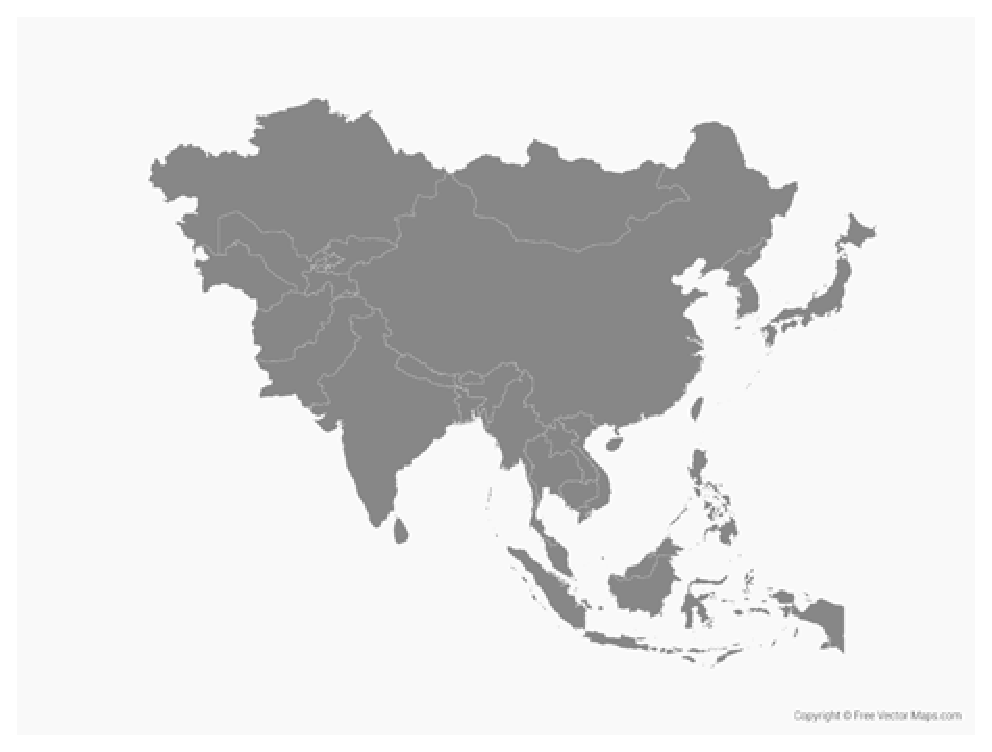
\includegraphics[width=0.85\textwidth,height=2.5cm,width=3.3cm]{asia.eps}
   
    \end{subfigure}
 
        \begin{subfigure}{0.4\textwidth}
        \includegraphics[width=0.85\textwidth,height=4cm]{US.eps}
        %\includegraphics[width=0.85\textwidth]{p1.png}
        \caption{USA}
        ~
        \end{subfigure}
        \begin{subfigure}{0.4\textwidth}
        \includegraphics[width=0.85\textwidth,height=3.5
        cm]{Asia.eps}
        \caption{Asia}
    \end{subfigure}        
    \end{figure}
   
 
 \end{frame}
 
 
 
    \begin{frame}
        \frametitle{Frequency of harasser roles}
        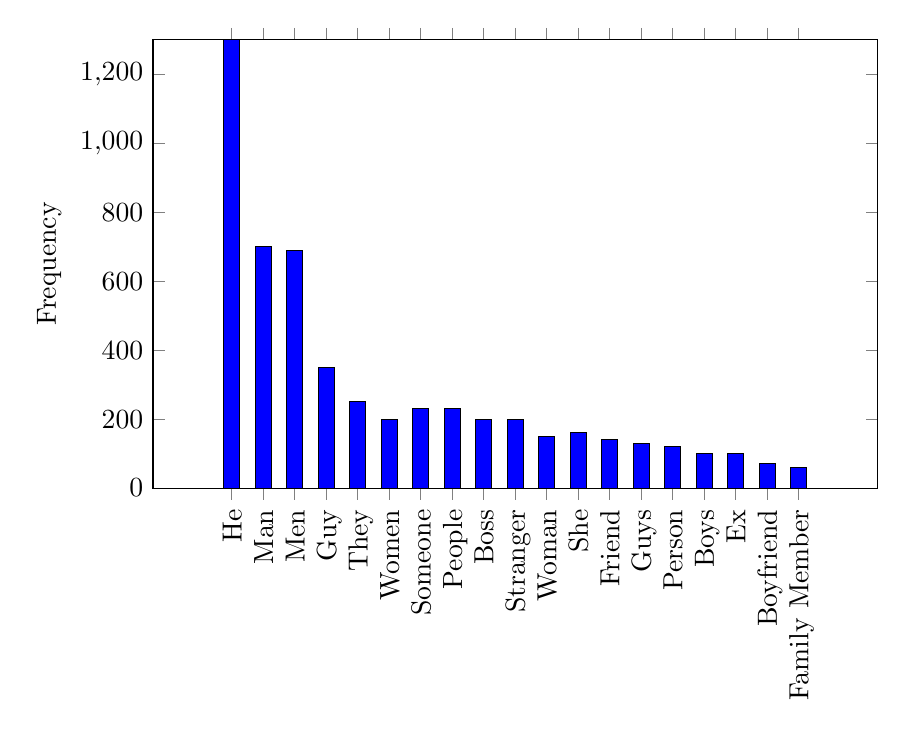
\begin{tikzpicture}
        \begin{axis}[
        ybar,
        bar width=.2cm, % Width of the bar
        x=.4cm, % Distance between the centers of the bars
        enlarge x limits={abs=1cm}, % The distance between the center of the first bar and the left edge
        enlarge y limits=false,
        ymin=0,
        xtick=data,
        xlabel=,
        symbolic x coords={He,Man,Men,Guy,They,Women,Someone,People,Boss,Stranger,Woman,She,Friend,Guys,Person,Boys,Ex,Boyfriend,Family Member},
        xtick=data,
        ylabel=Frequency,
        xticklabel style={text height=0ex},
        xticklabel style={rotate=90,anchor=north east},
        %ymajorgrids,yminorgrids,minor y tick num=4,
        ]
       
       
        \addplot[ybar,fill=blue] coordinates {
            (He,1300)(Man,700)(Men,690)(Guy,350)(They,250)(Women,200)(Someone,230)(People,230)(Boss,200)(Stranger,200)(Woman,150)
            (She,160)(Friend,140)(Guys,130)(Person,120)(Boys,100)(Ex,100)(Boyfriend,70)(Family Member,60)
        };
       
       
        \end{axis}
       
       
        \end{tikzpicture}
    \end{frame}
\begin{frame}
        \frametitle{Limitations}
        \begin{itemize}
            \item Findings may not be generalized \pause
            \item Not the representation of the whole movement \pause
            \item Misrepresentation on social media \pause
           
           
           
        \end{itemize}
\end{frame}
\end{document}